%%%%%%%%%%%%
%%
%%%%%%%%%%%%

\section{Background}

\subsection{Core PROV model} \label{sec:prov-core}

We now introduce the core elements of the PROV model, which forms the basis for the grouping operator.
%
We maintain a dual view of provenance, both as a relational model (with binary relations) and as a graph model. Viewed as a relational model, PROV includes three types of elements: Entities ($\en$), Activities ($\act$), and Agents ($\ag$), and several types of relations amongst them. 
In line with the description in~\citep{w3c-prov-dm} (sec. 2), PROV is defined by the following core relations, with common abbreviations in brackets. 

\begin{eqnarray*}
Used~~(\used)  & \subseteq & \act \times \en \\
WasGeneratedBy~~(\wgby) & \subseteq  & \en \times \act \\
WasDerivedFrom~~(\wdf) & \subseteq   & \en \times \en \\
WasInvalidatedBy~~(\inv) &  \subseteq &  \en \times \act \\
WasAssociatedWith~~(\waw) & \subseteq & \act \times \ag \\
ActedOnBehalfOg~~(\delegate) & \subseteq & \ag \times \ag \\ 
WasAttributedTo~~(\attrTo) & \subseteq & \en \times \ag \\
WasInformedBy~~(\wasInfBy) & \subseteq & \act \times \act
\end{eqnarray*}


% \begin{figure}
% \centering
% 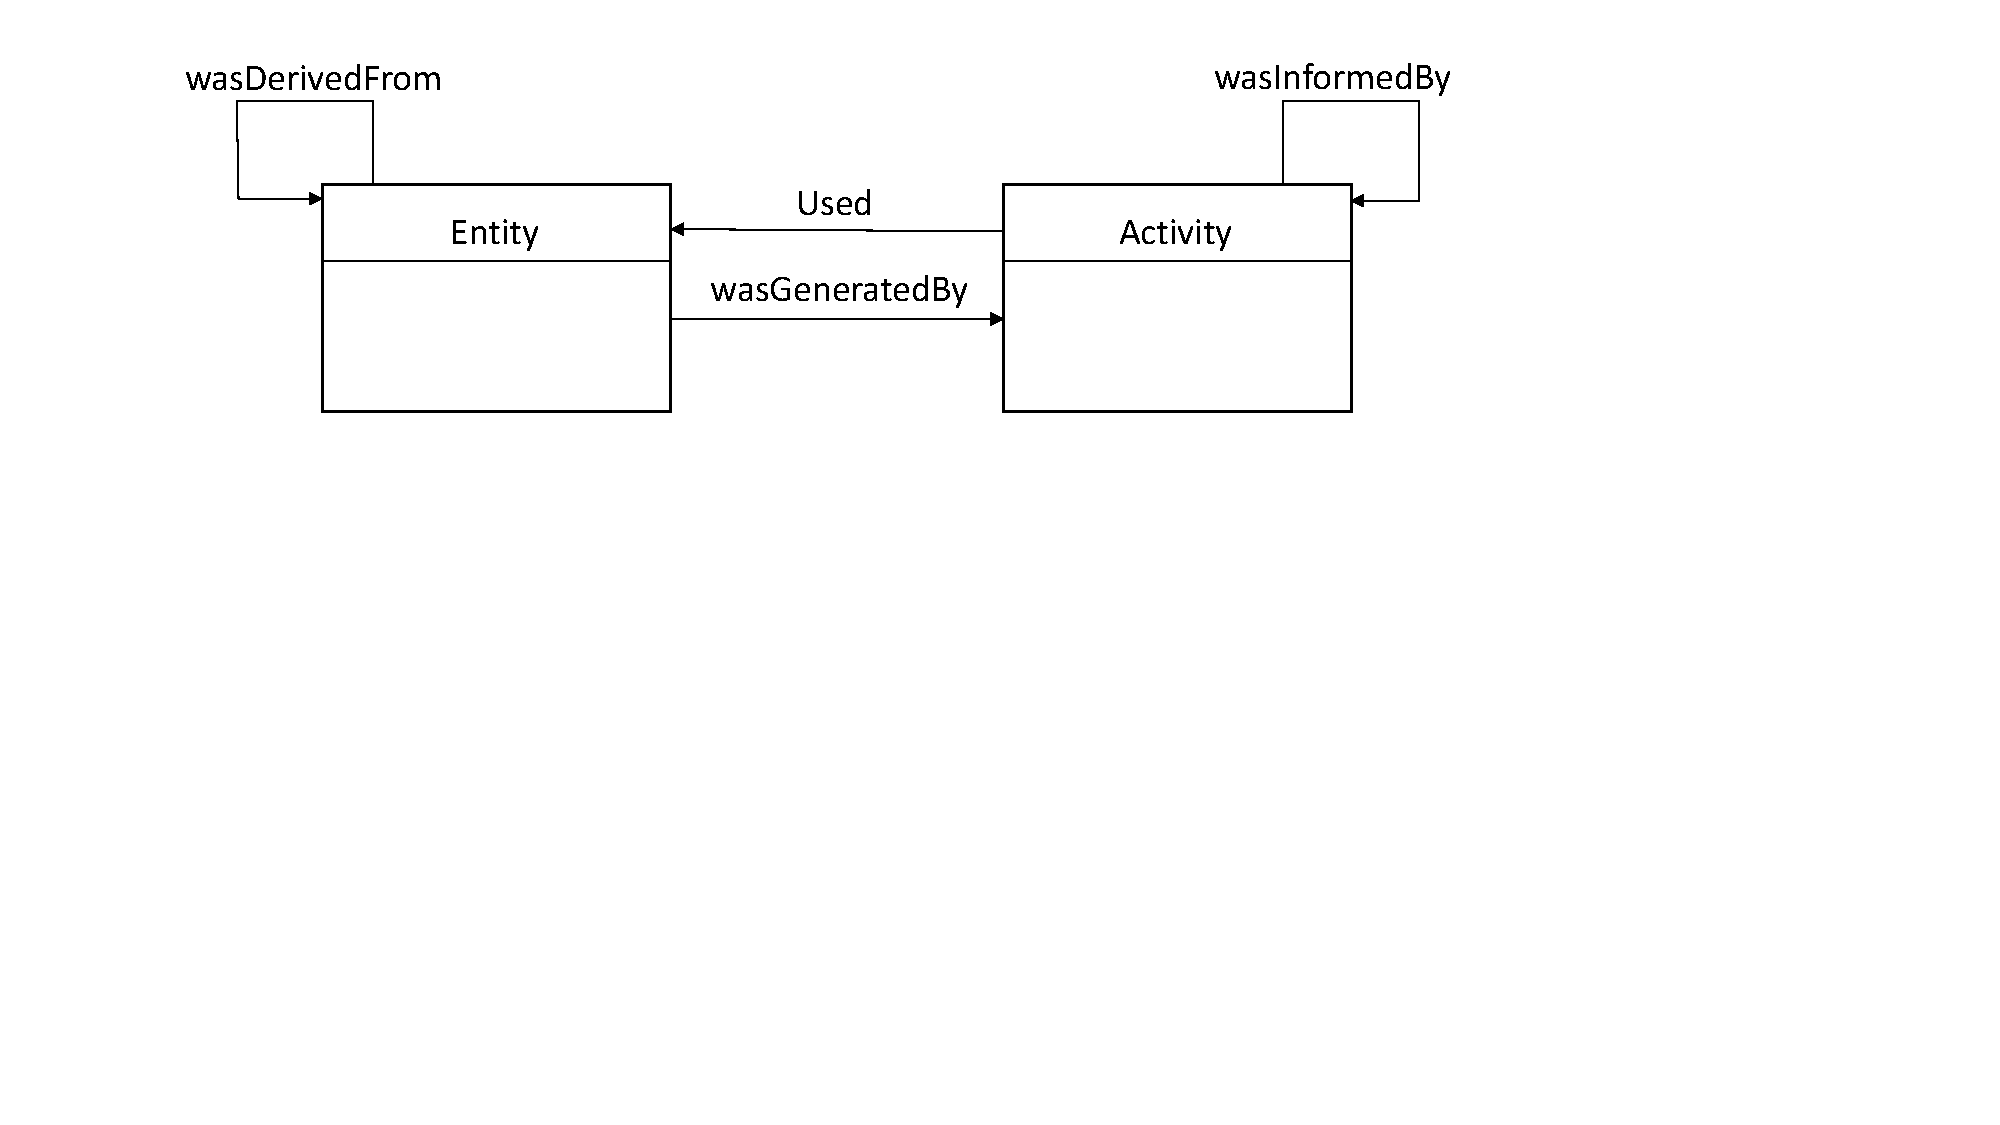
\includegraphics[scale=.45]{figures/prov-essentials.pdf} 
% \caption{Core elements of the PROV model, adapted from~\citep{w3c-prov-dm}}
% \label{fig:prov-core}
%  \end{figure}
% %

%\subsection{Bipartite PROV: $\guEA$}  \label{sec:prov-guea}
%These are summarized in Fig.~\ref{fig:prov-core}.
%
Initially, we are going to restrict ourselves to an even simpler model, consisting only of $\en$, $\act$, and relations $\used$ and $\wgby$.
%Agents and the relations that involve them are introduced in Sec.~\ref{sec:agents-abstraction}.
%
%Further extensions to the additional relations --- $\wdf$ and $\wasInfBy$ --- are straightforward and are not considered in detail.

%
An instance  of the model is a provenance document $D$, consisting of sets $en \in \en$ and $act \in \act$ of symbols, and sets of relation instances $\{ \wgby(e,a)  | e \in \en, a \in \act \} \cup   \{ \used(a,e)  | e \in \en, a \in \act\}$. 

%
As these relations are binary, we view $D$ as a digraph $G=(V,E)$, where $V= \en \cup \act$, and each relation instance maps to a labelled directed edge. By convention, we orient these edges from right to left, to denote that the relation ``points back to the past''. Thus:
$a \xleftarrow{\wgby} e \in E$ iff $\wgby(e,a) \in D$, and $e \xleftarrow{\used} a \in E$ iff $\used(a,e) \in D$.
%
We denote the label associated to edge $(v_i, v_j)$ as $\elabel(v_i,v_j)$. 

%
Note that, by definition of the relations, $G$ is a bipartite graph.
We denote the set of all such graphs, containing only $\en$ and $\act$ nodes, and $\wgby$ and $\used$ edges,  by $PG$. 
%In Sec.~\ref{sec:agents-abstraction} we are going to extend this set to include agents as well as additional relations.
%Fig.{fig:baseline-ug-ae} portrays a simple $\guEA$ graph that we will be using as a running example.

% \begin{figure}
% \centering
% 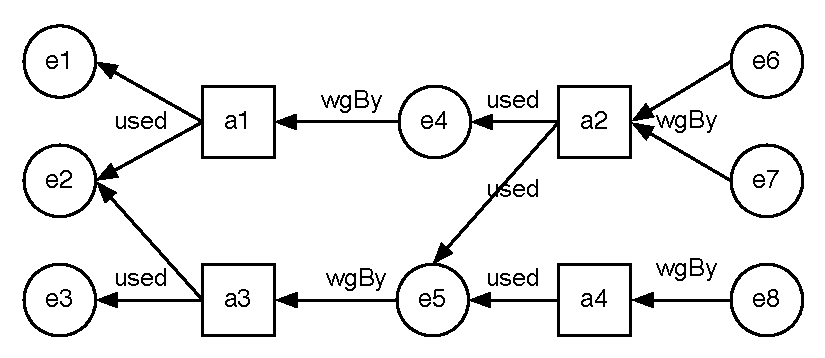
\includegraphics[scale=.6]{figures/baseline-ug-ae.pdf} 
% \caption{$\guEA$ provenance graph used as a running example to illustrate abstraction by grouping}  \label{fig:baseline-ug-ae}
% \end{figure}
% 
